
% Copyright 2019 Clara Eleonore Pavillet

% Author: Clara Eleonore Pavillet
% Description: This is an unofficial Oxford University Beamer Template I made from scratch. Feel free to use it, modify it, share it.
% Version: 1.0

\documentclass{beamer}
% Load Packages
\usepackage[utf8]{inputenc}
\usepackage{xcolor}
\usepackage{tikz}
\usetikzlibrary{positioning,calc}
\usepackage{graphicx}
\usepackage{hyperref}
\usepackage{amsmath}
\usepackage{listings}
\usepackage{fontawesome}

% Define Commands
\newcommand*{\ClipSep}{0.06cm} %To adjust footer logo
\newcommand{\E}{\mathrm{e}\,} %\def\I{e} % used to defined e for exp(x), see later what it should be
\newcommand{\ud}{\mathrm{d}}
\lstset{numbers=left, numberstyle=\tiny, stepnumber=1,firstnumber=1,breaklines=true,
    numbersep=5pt,language=Python,
    stringstyle=\ttfamily,
    basicstyle=\footnotesize, 
    showstringspaces=false
}

\usetheme{oxonian}

\title{Predicting COVID Moonshot molecule binding affinity}
\titlegraphic{
\includegraphics[width=2cm]{Theme/Logos/OxfordLogoV1.png}}
\author{Isaac Ellmen \& Sim Zhao}
\institute{University of Oxford}
\date{} %\today

\begin{document}

{\setbeamertemplate{footline}{} 
\frame{\titlepage}}
    

\subsection{Introduction}
\begin{frame}{Introduction}

\begin{enumerate}
    \item Determine binding affinity of putative SARS-CoV-2 protease binders
    \item Strong focus on workflow automation
    \item Snakemake powers the entire process
\end{enumerate}
    
\end{frame}
    

\subsection{Our workflow DAG}
\begin{frame}{Our workflow DAG}

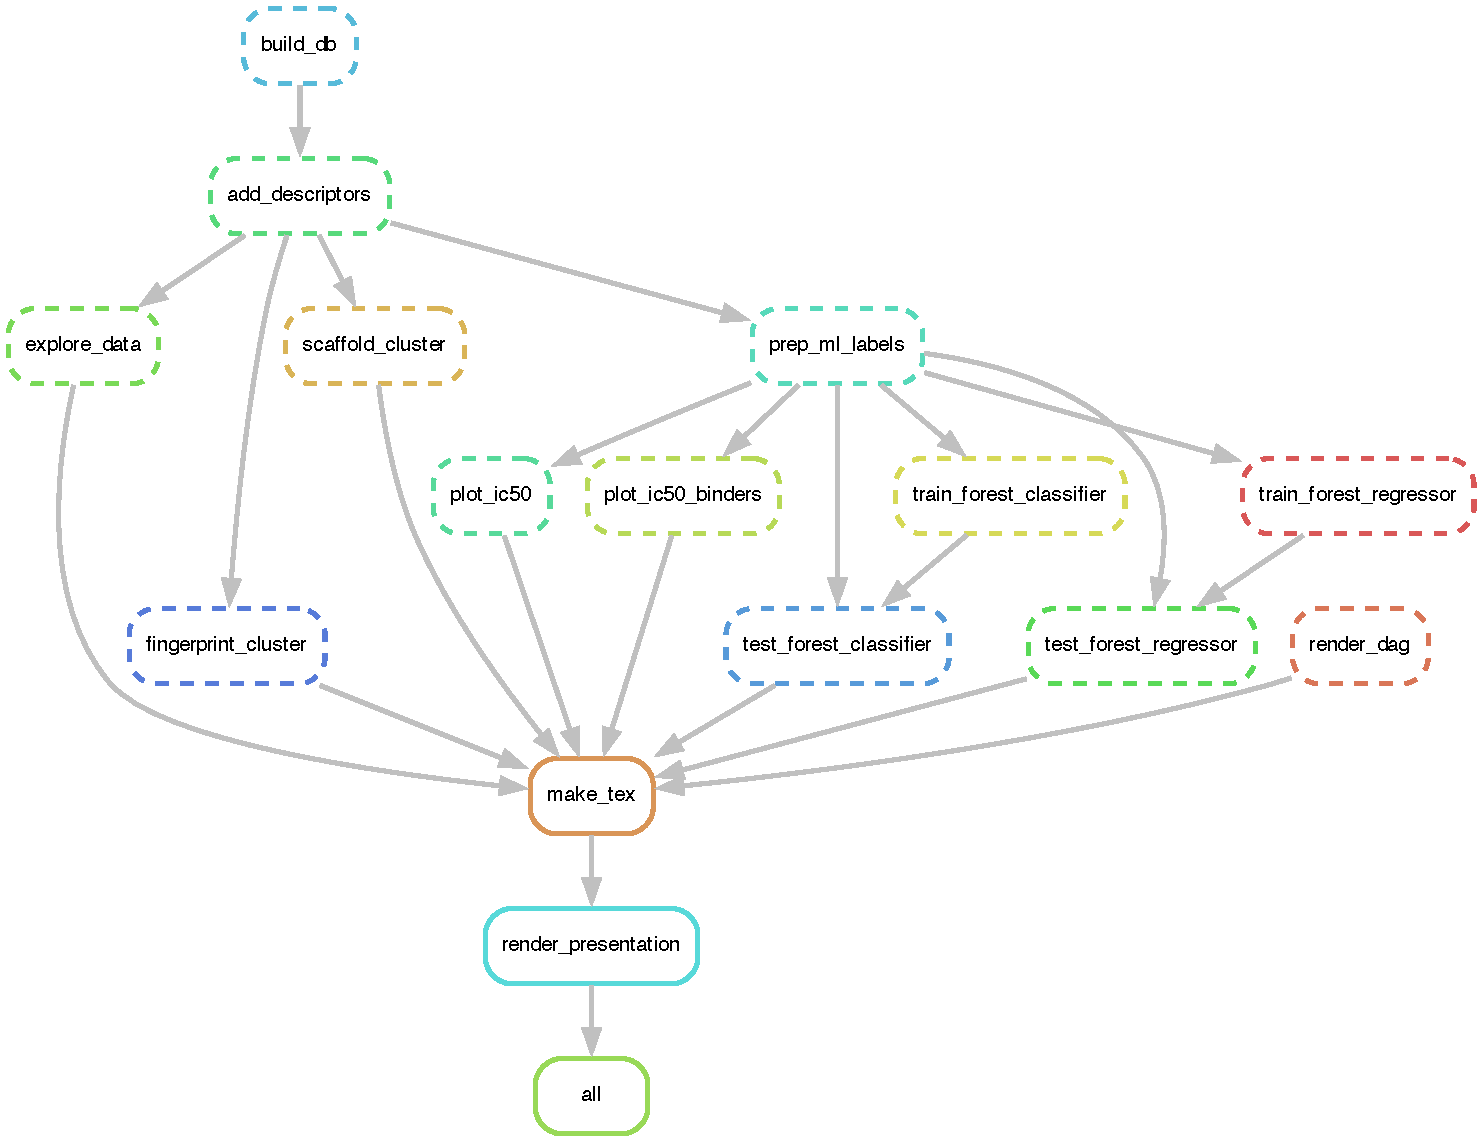
\includegraphics[width=0.9\textwidth]{../outputs/dag.pdf}
    
\end{frame}
    

\subsection{Building the SQLite DB}
\begin{frame}[fragile]{Building the SQLite DB}

\begin{block}{Build database}
\begin{lstlisting}[firstnumber=1, label=glabels, xleftmargin=10pt] 
import sqlite3
import pandas as pd

def build_db(data_path, out_path):
    con = sqlite3.connect(out_path)
    cur = con.cursor()
    df = pd.read_csv(data_path, index_col='CID')
    assays_df = df.drop(columns=['SMILES'])
    compounds_df = df[['SMILES']]
    assays_table = 'assays'
    assays_df.to_sql(assays_table, con, if_exists='replace', index=True)
    compounds_table = 'compounds'
    compounds_df.to_sql(compounds_table, con, if_exists='replace', index=True)
    con.close()

\end{lstlisting}
\end{block}
    
\end{frame}
    

\subsection{Fingerprint clustering - sensitivity to cutoff}
\begin{frame}{Fingerprint clustering - sensitivity to cutoff}

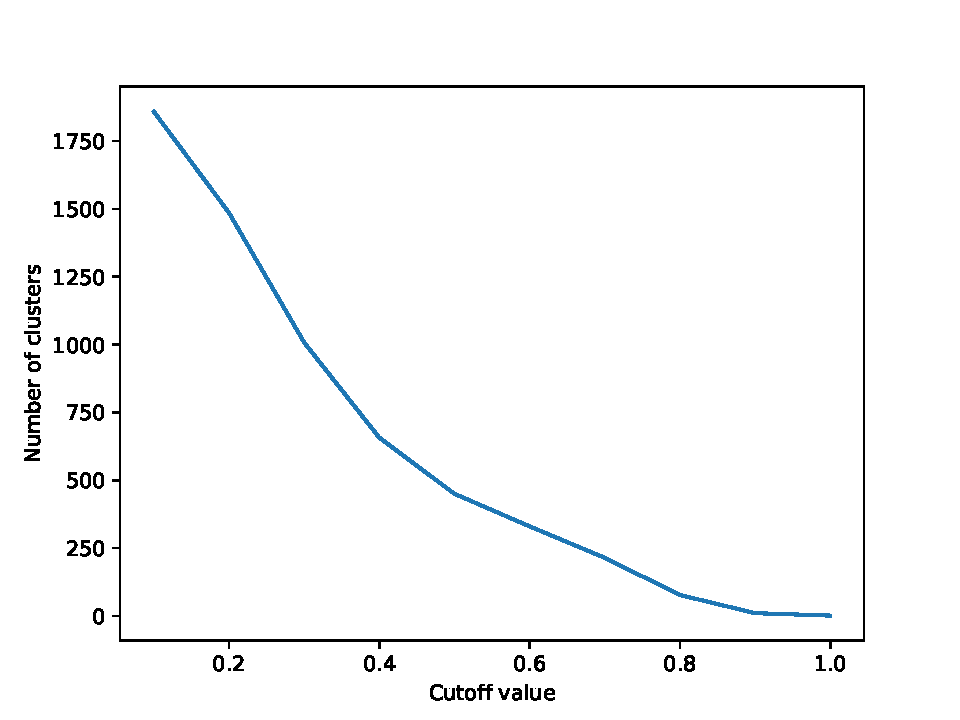
\includegraphics[width=0.9\textwidth]{../outputs/fingerprint_cluster_cutoffs.pdf}
    
\end{frame}
    

\subsection{Fingerprint clustering - class composition}
\begin{frame}{Fingerprint clustering - class composition}

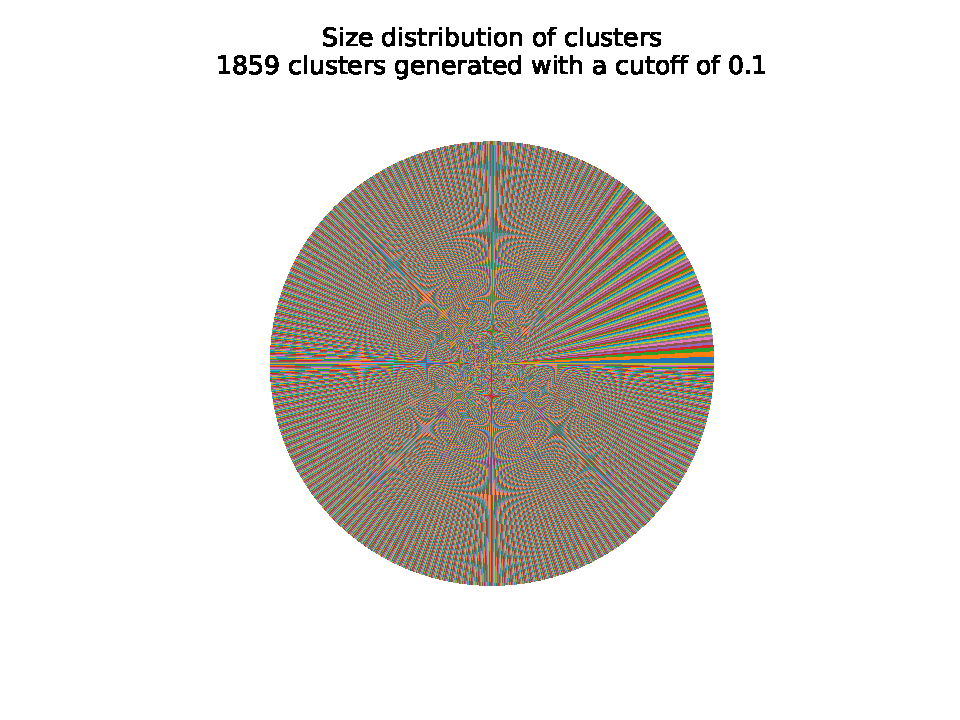
\includegraphics[width=0.3\textwidth]{../outputs/fingerprint_clusters_0.1.pdf}
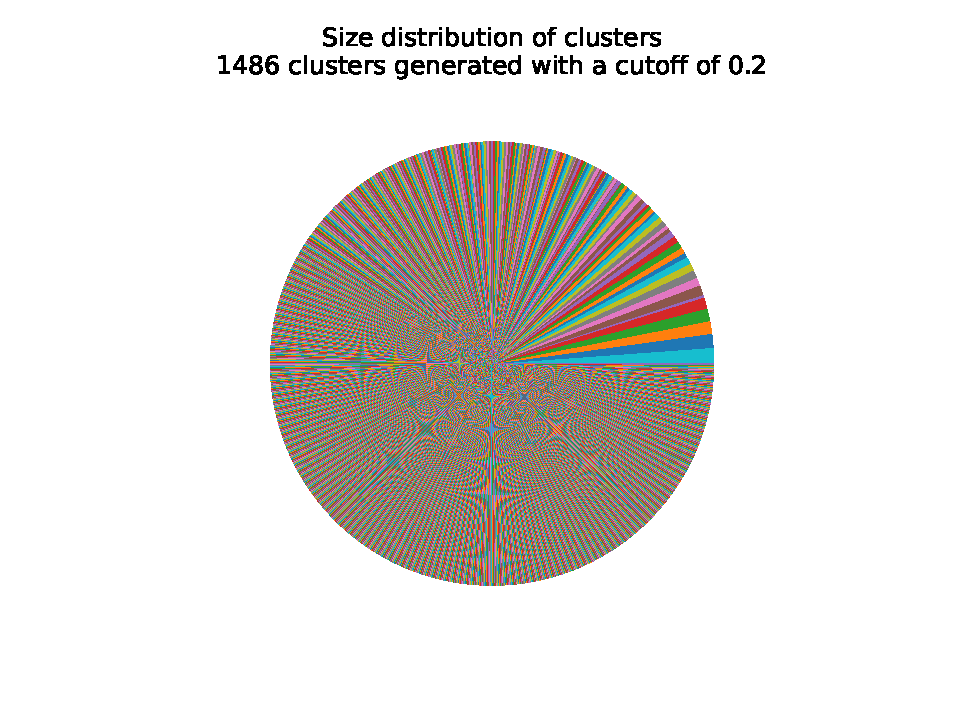
\includegraphics[width=0.3\textwidth]{../outputs/fingerprint_clusters_0.2.pdf}
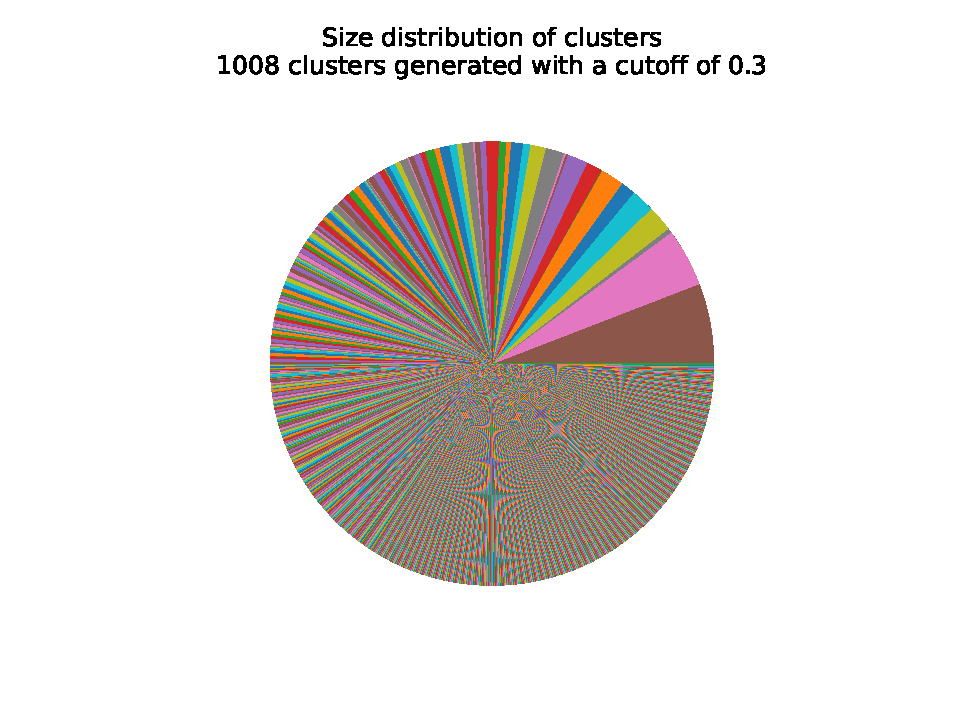
\includegraphics[width=0.3\textwidth]{../outputs/fingerprint_clusters_0.3.pdf}
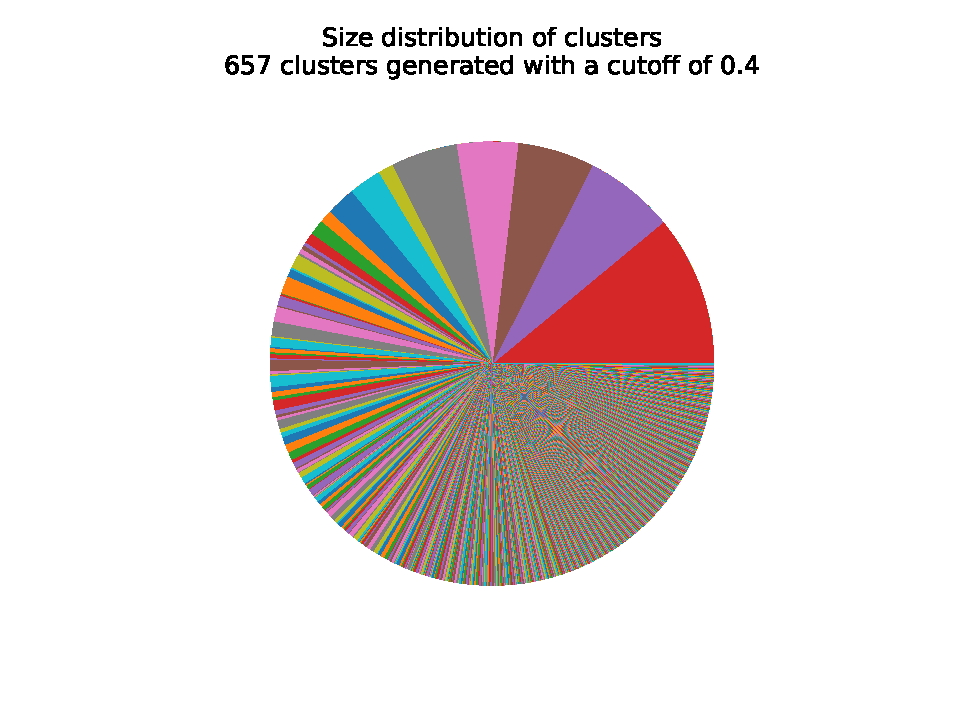
\includegraphics[width=0.3\textwidth]{../outputs/fingerprint_clusters_0.4.pdf}
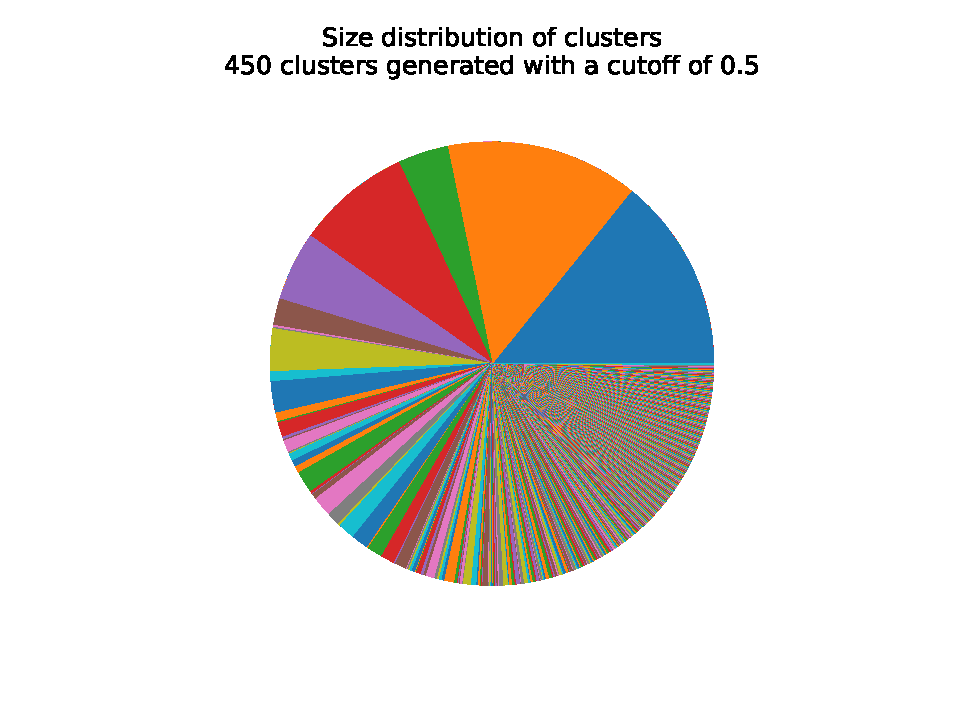
\includegraphics[width=0.3\textwidth]{../outputs/fingerprint_clusters_0.5.pdf}
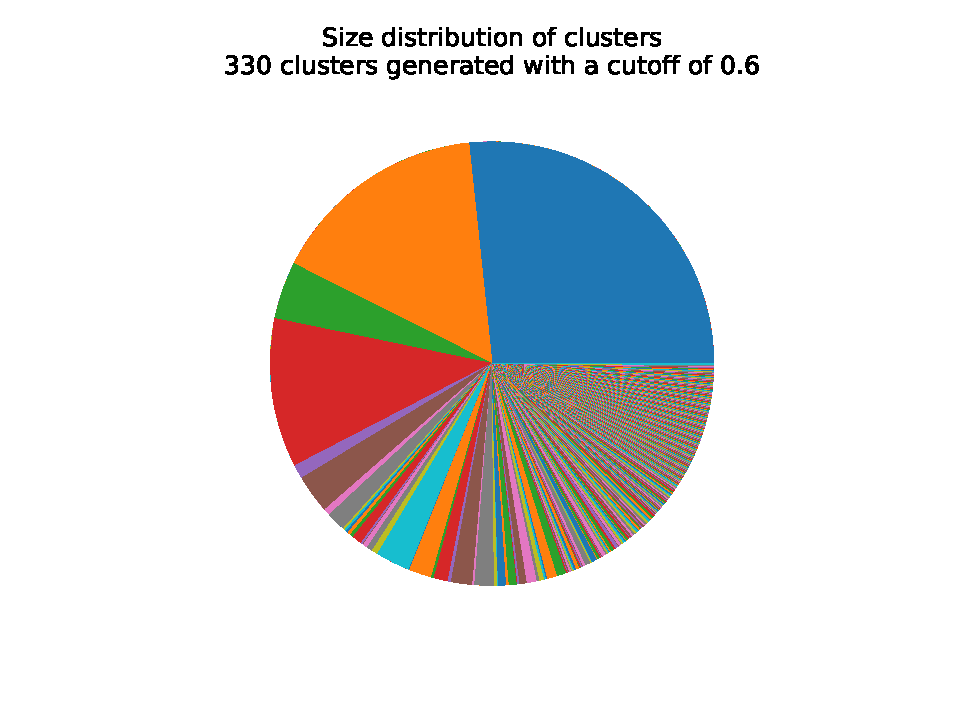
\includegraphics[width=0.3\textwidth]{../outputs/fingerprint_clusters_0.6.pdf}
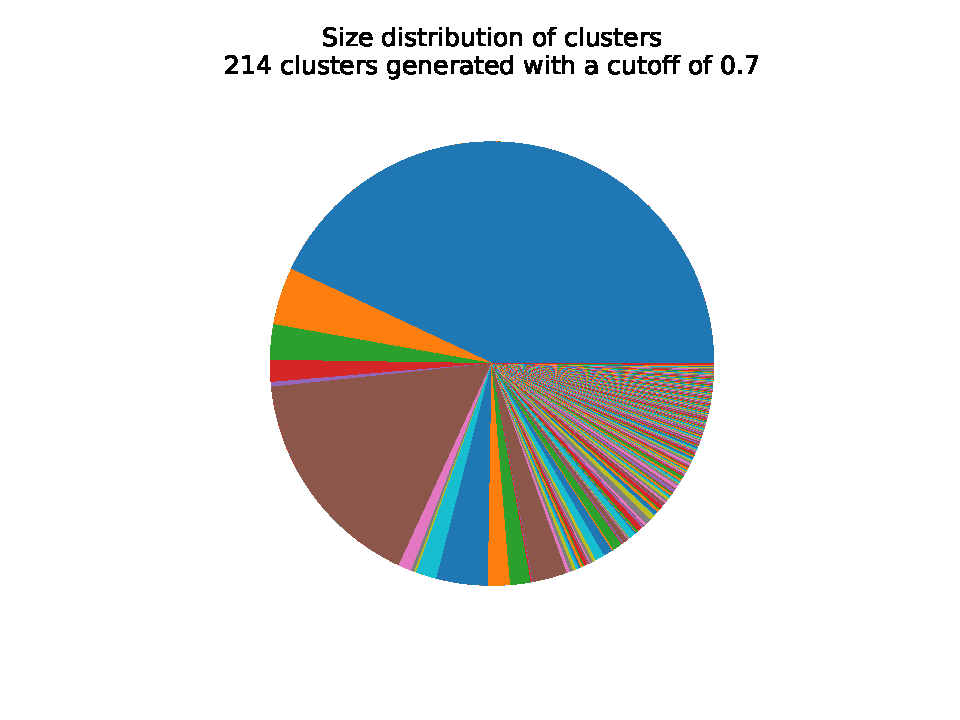
\includegraphics[width=0.3\textwidth]{../outputs/fingerprint_clusters_0.7.pdf}
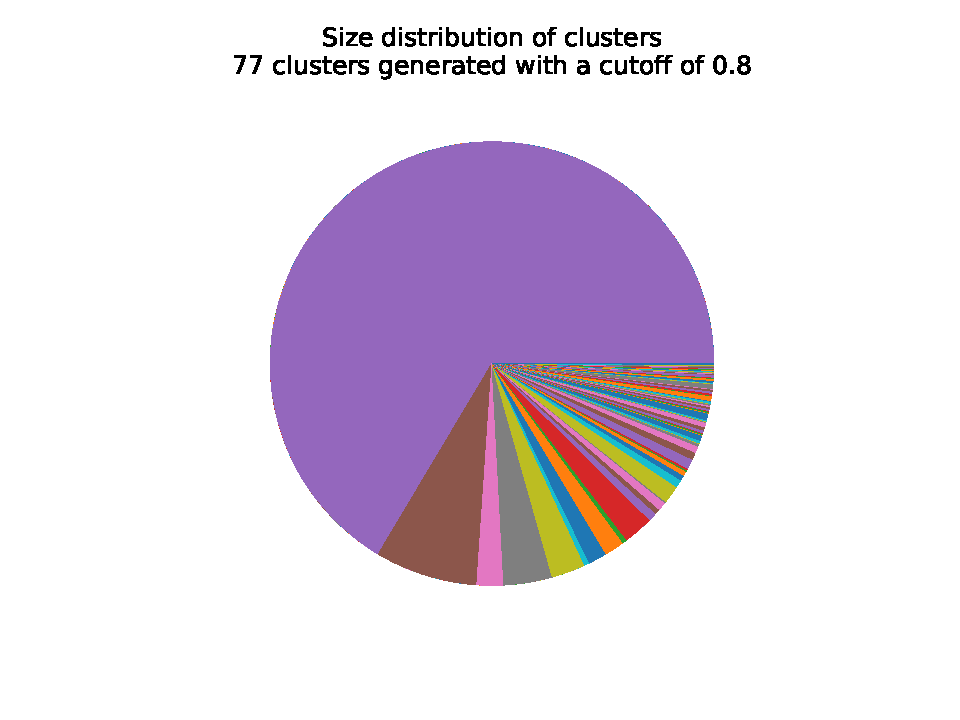
\includegraphics[width=0.3\textwidth]{../outputs/fingerprint_clusters_0.8.pdf}
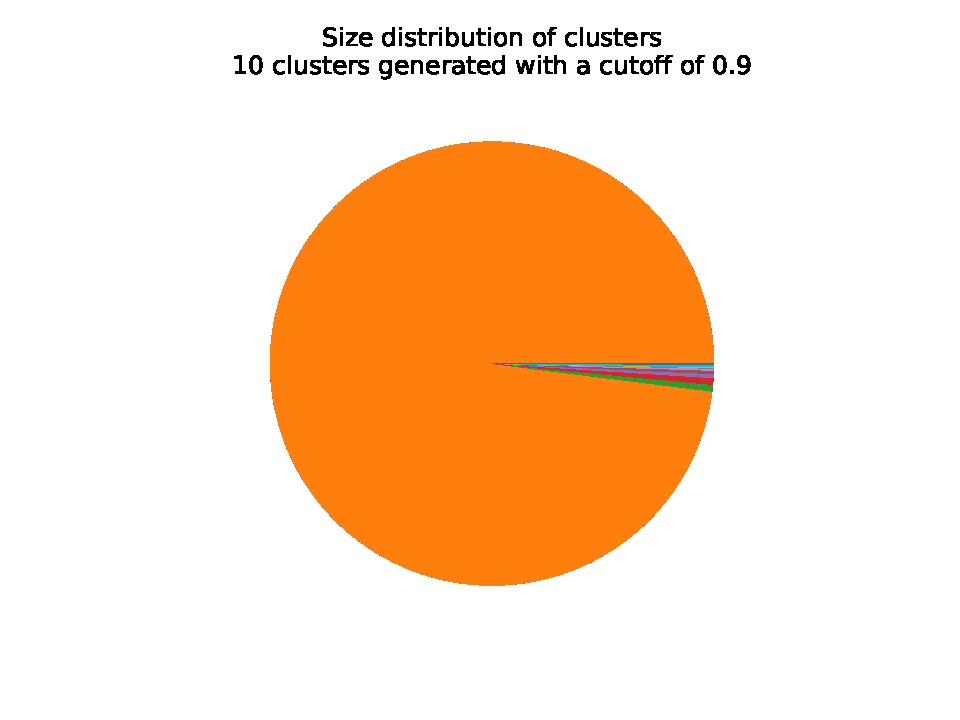
\includegraphics[width=0.3\textwidth]{../outputs/fingerprint_clusters_0.9.pdf}
    
\end{frame}
    

\subsection{Scaffold clustering - sensitivity to cutoff}
\begin{frame}{Scaffold clustering - sensitivity to cutoff}

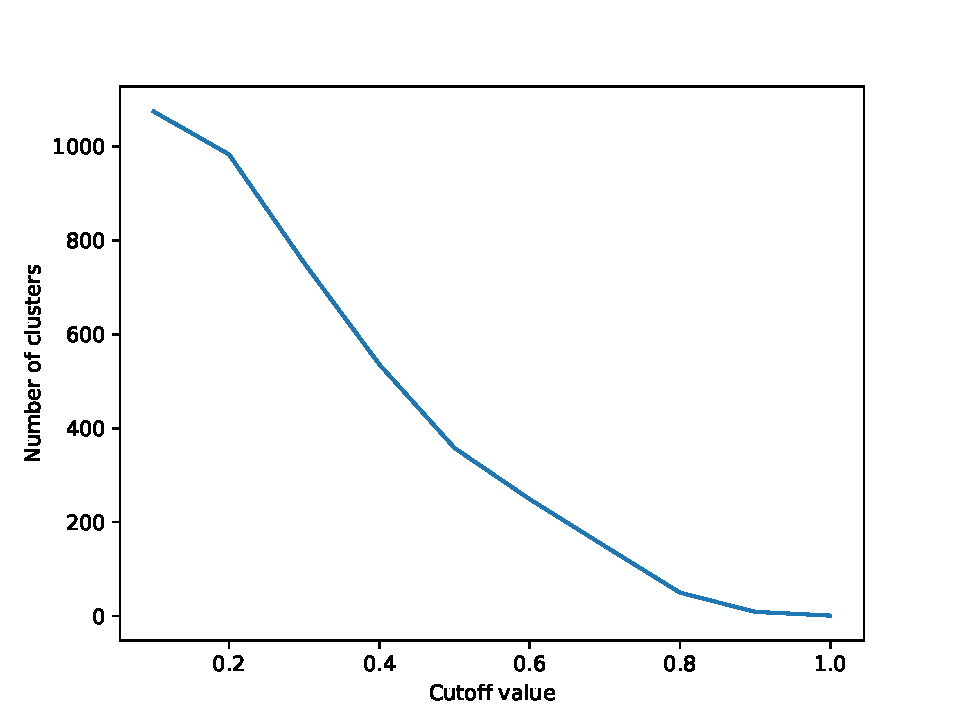
\includegraphics[width=0.9\textwidth]{../outputs/scaffold_cluster_cutoffs.pdf}
    
\end{frame}
    

\subsection{Scaffold clustering - class composition}
\begin{frame}{Scaffold clustering - class composition}

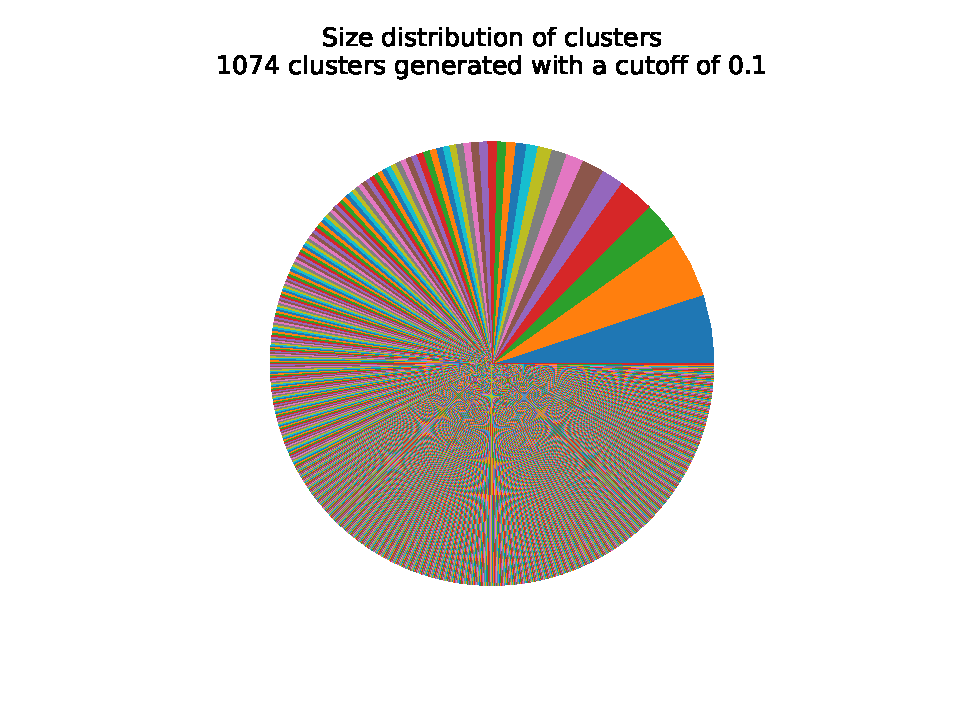
\includegraphics[width=0.3\textwidth]{../outputs/scaffold_clusters_0.1.pdf}
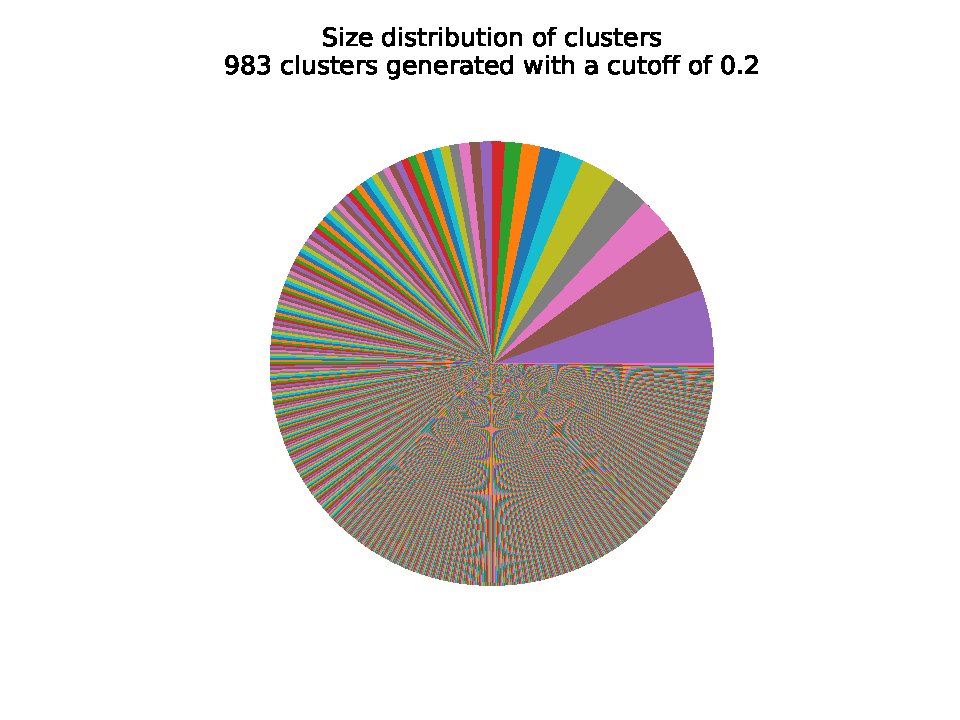
\includegraphics[width=0.3\textwidth]{../outputs/scaffold_clusters_0.2.pdf}
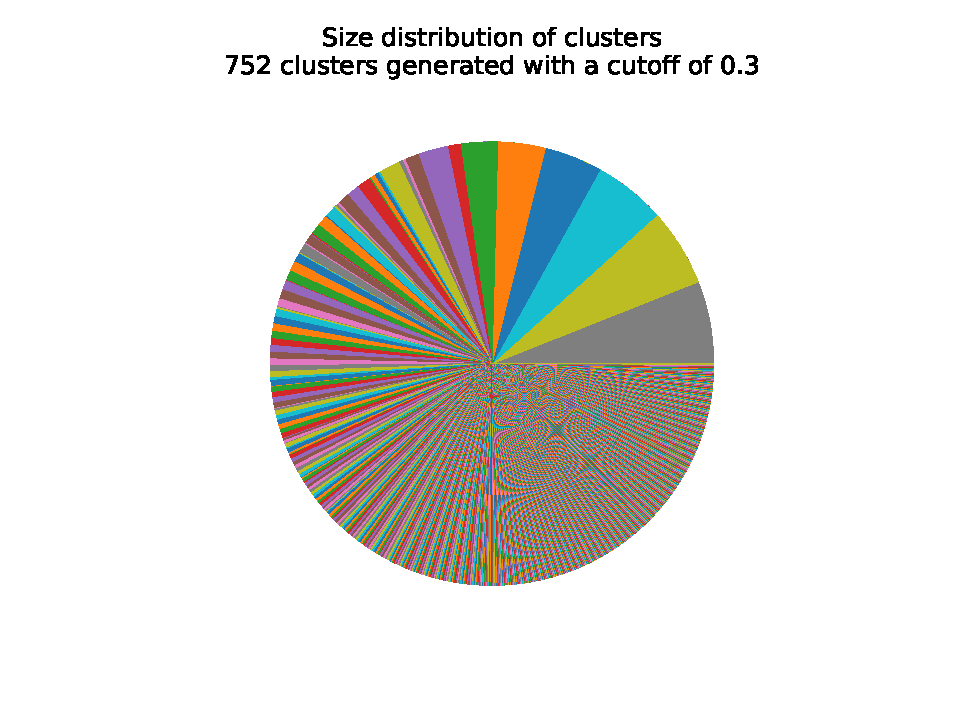
\includegraphics[width=0.3\textwidth]{../outputs/scaffold_clusters_0.3.pdf}
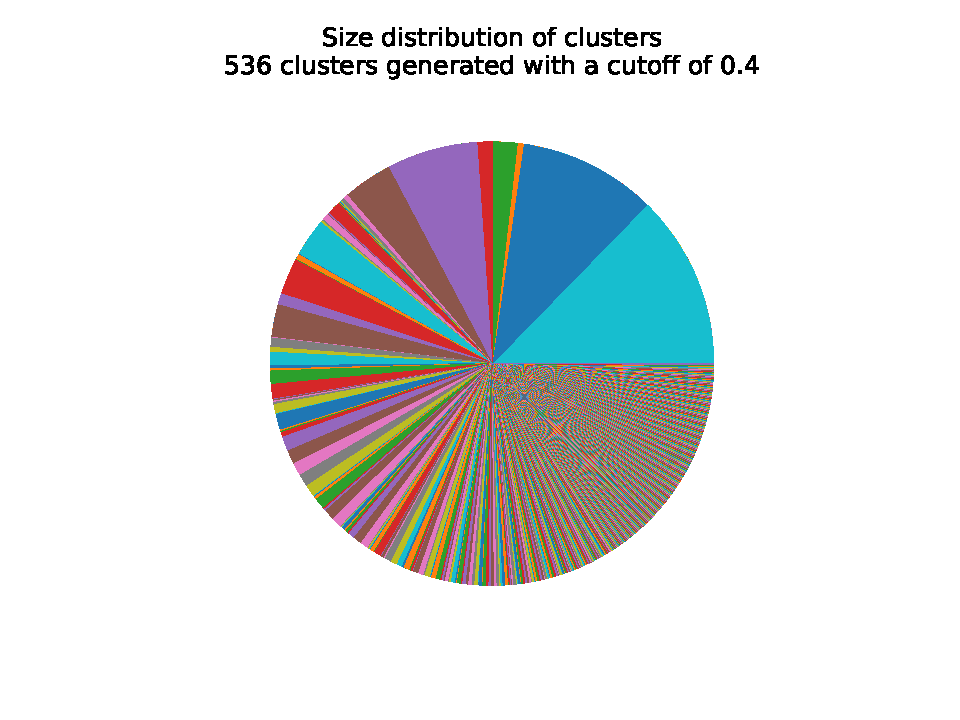
\includegraphics[width=0.3\textwidth]{../outputs/scaffold_clusters_0.4.pdf}
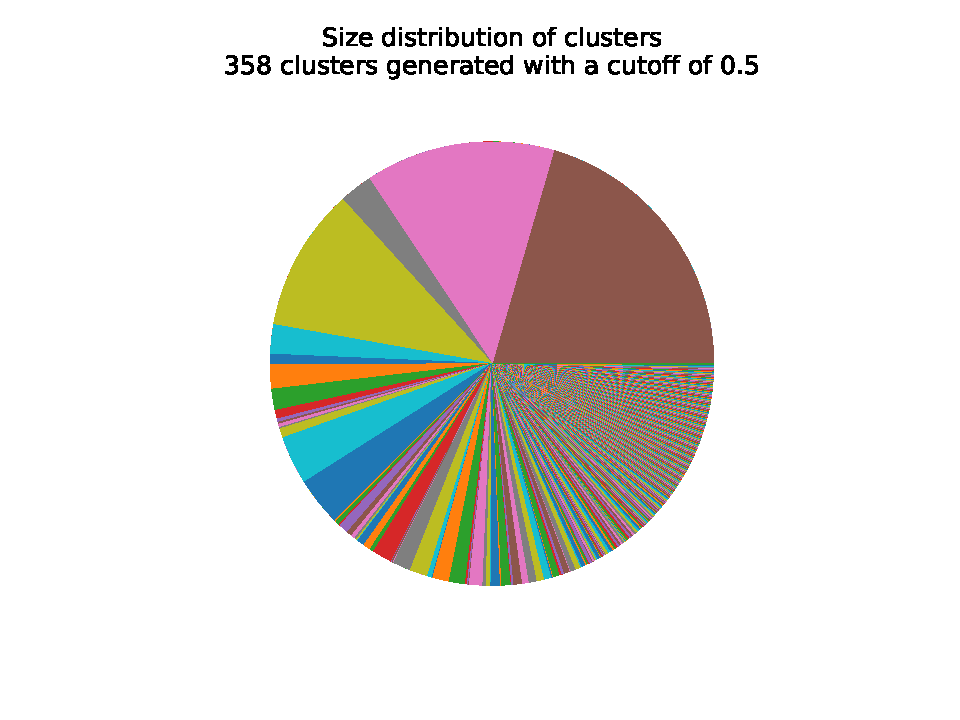
\includegraphics[width=0.3\textwidth]{../outputs/scaffold_clusters_0.5.pdf}
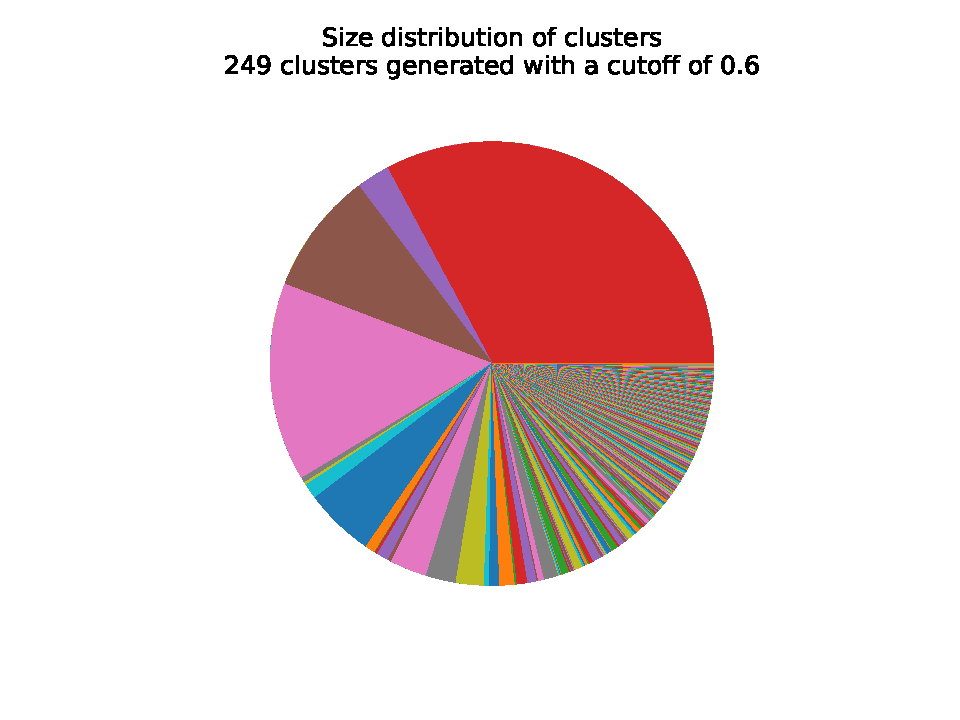
\includegraphics[width=0.3\textwidth]{../outputs/scaffold_clusters_0.6.pdf}
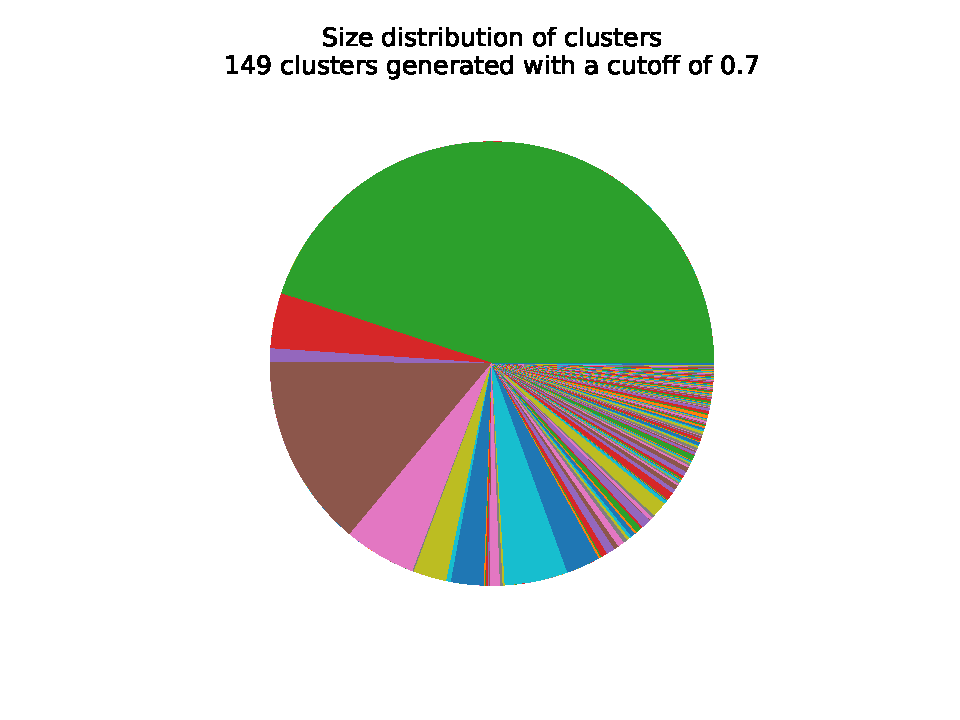
\includegraphics[width=0.3\textwidth]{../outputs/scaffold_clusters_0.7.pdf}
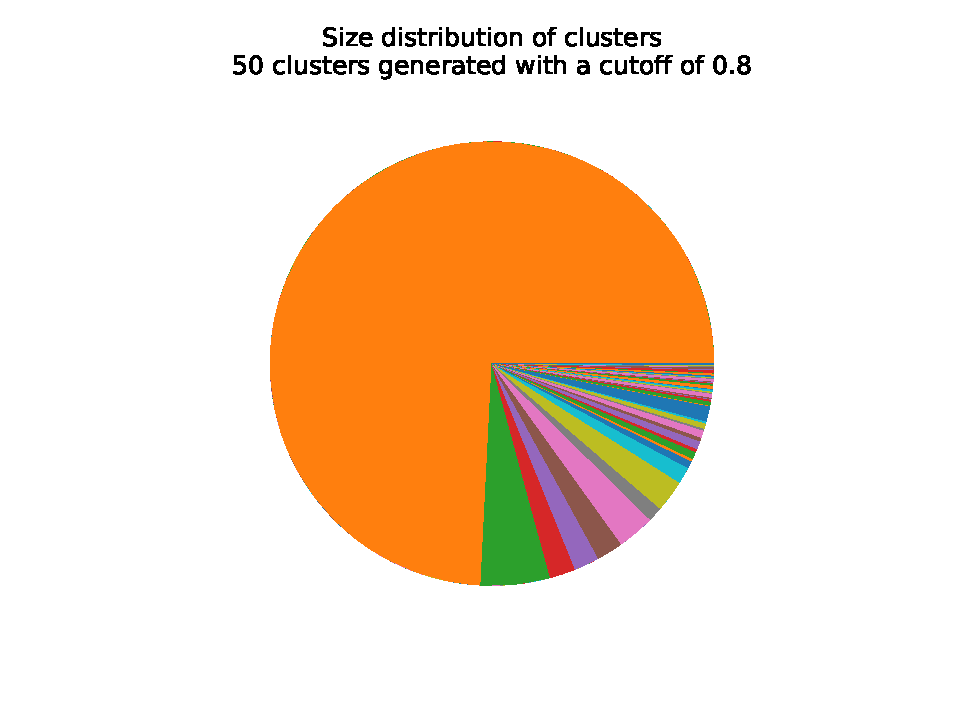
\includegraphics[width=0.3\textwidth]{../outputs/scaffold_clusters_0.8.pdf}
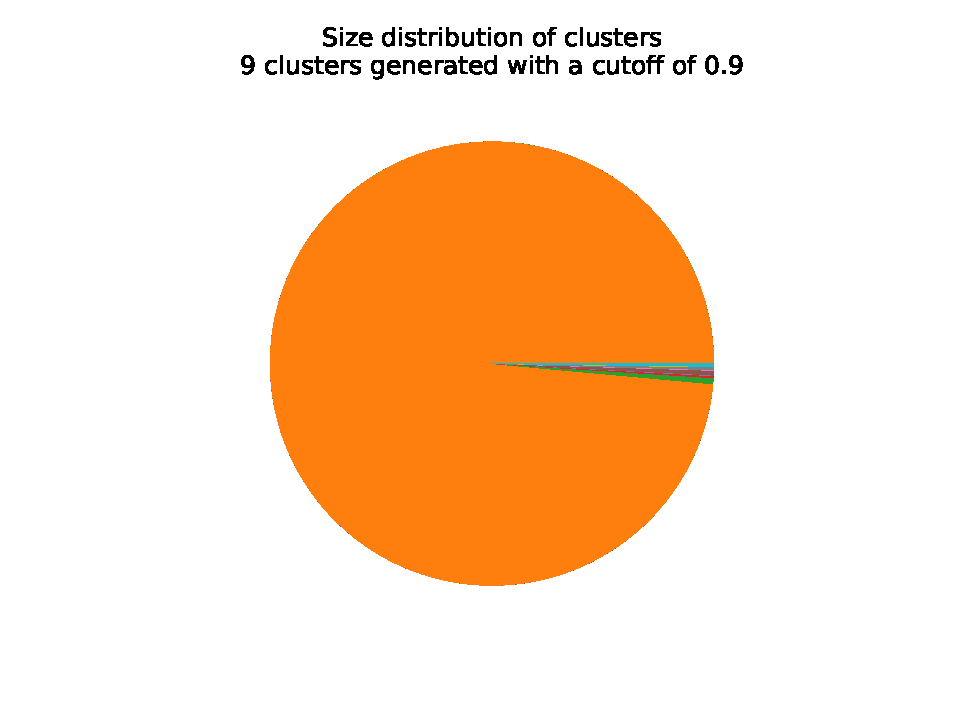
\includegraphics[width=0.3\textwidth]{../outputs/scaffold_clusters_0.9.pdf}
    
\end{frame}
    

\subsection{pIC50 distribution}
\begin{frame}{pIC50 distribution}

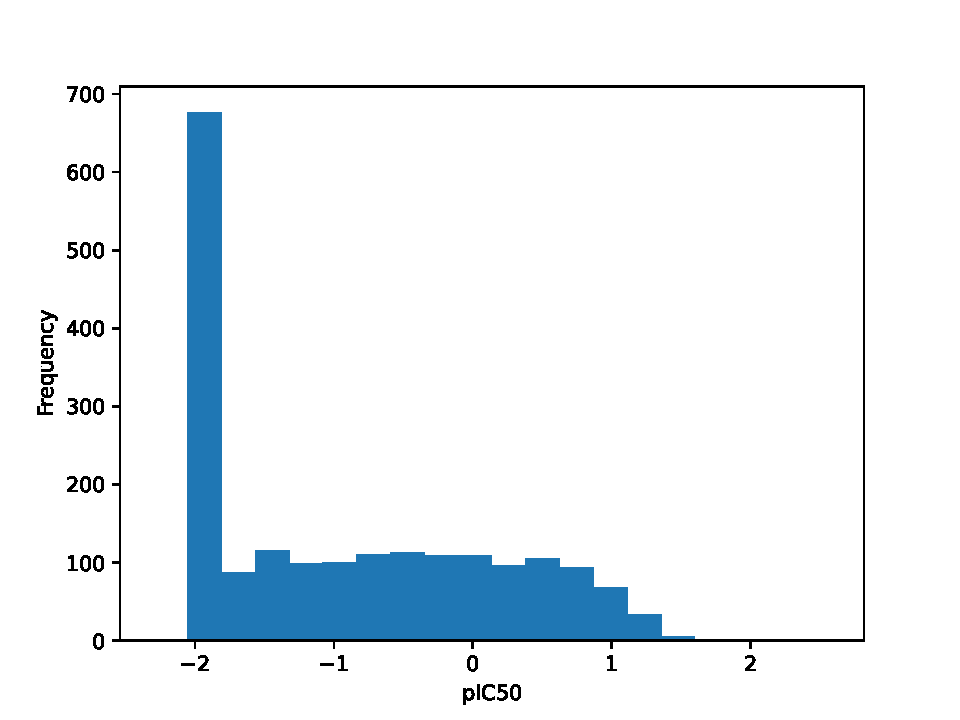
\includegraphics[width=0.9\textwidth]{../outputs/ic50_distribution.pdf}
    
\end{frame}
    

\subsection{pIC50 distribution (only binders)}
\begin{frame}{pIC50 distribution (only binders)}

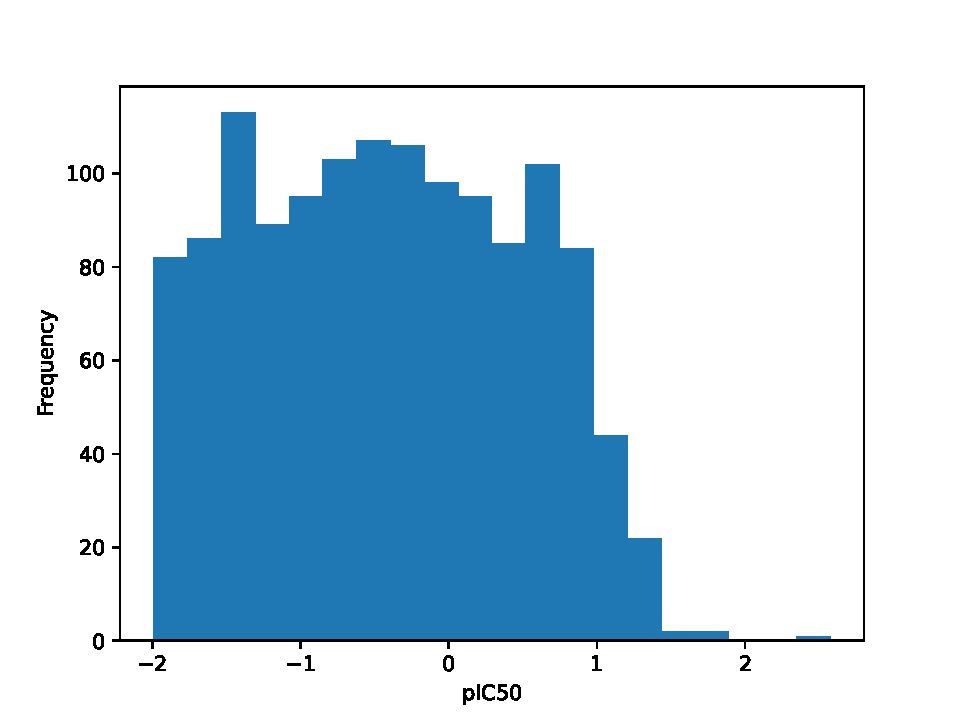
\includegraphics[width=0.9\textwidth]{../outputs/ic50_binders_distribution.pdf}
    
\end{frame}
    

\subsection{Strategy}
\begin{frame}{Strategy}

\begin{enumerate}
    \item Classification for binders vs. non-binders
    \item Regression for binding strength (pIC50)
    \item Can use similar model for both since learning very similar properties
\end{enumerate}
    
\end{frame}
    

\subsection{Compute descriptors}
\begin{frame}[fragile]{Compute descriptors}

\begin{block}{Compute Descriptors}
\begin{lstlisting}[firstnumber=1, label=glabels, xleftmargin=10pt] 
def compute_descriptors(molecule):
    descriptors ={}
    for d in Descriptors.descList:
        try:
            value = d[1](molecule)
            descriptors[d[0]] = value

        except:
            value = np.nan
            descriptors[d[0]] = np.nan
    descriptors = pd.Series(descriptors)
    return descriptors

\end{lstlisting}
\end{block}
    
\end{frame}
    

\subsection{Make dataframe}
\begin{frame}[fragile]{Make dataframe}

\begin{block}{Make Dataframe}
\begin{lstlisting}[firstnumber=1, label=glabels, xleftmargin=10pt] 
def pack_df(df_with_SMILES):
    descriptorsdf = pd.DataFrame()
    for index, row in df_with_SMILES.iterrows():
    # Get the SMILES string of the compound
        smiles = row['SMILES']
    # Create a rdkit molecule object from SMILES
        mol = Chem.MolFromSmiles(smiles)
        des = compute_descriptors(mol)
        for i in range(len(des)):
                descriptorsdf.at[index,'{}'.format(des.index[i])] = des.values[i]
    return descriptorsdf

\end{lstlisting}
\end{block}
    
\end{frame}
    

\subsection{Feature selection}
\begin{frame}[fragile]{Feature selection}

\begin{block}{Feature Selection}
\begin{lstlisting}[firstnumber=1, label=glabels, xleftmargin=10pt] 
def feature_selection(Descriptors_df, y_df, k_feature = 10, task = 'regress', way = 'simple', rfe_step = 0.2):
    if task == 'regress':
        estimator = SVR(kernel="linear")
    if task == 'classification':
        estimator = LogisticRegression()
    if way == 'simple':
        selector = SelectKBest(f_classif, k=k_feature)
    if wat == 'rfe':
        selector = RFE(estimator, n_features_to_select=k_feature, step=rfe_step)
    selector.fit(Descriptors_df, y_df)
    top_k_idx = selector.get_support(indices=True)
    return Descriptors_df.columns[top_k_idx]

\end{lstlisting}
\end{block}
    
\end{frame}
    

\subsection{Best 10 parameters}
\begin{frame}[fragile]{Best 10 parameters}

\setlength{\topsep}{3mm}
\begin{tabular}{|c|c|}
\hline
\textbf{Feature Descriptor} & \textbf{Meaning} \\ 
\hline

PEOE\_VSA8 & Polarizability based on Eigenvalues of the \\ & Overlap matrix (PEOE) with 8 VSA \\ 
\hline
fr\_N\_O & Nitro group \\ 
\hline
fr\_diazo & Diazo group \\ 
\hline
fr\_dihydropyridine & Dihydropyridine group \\ 
\hline
fr\_hdrzine & Hydrazine group \\ 
\hline
fr\_ketone\_Topliss & Ketone group using Topliss method \\ 
\hline
fr\_lactam & Lactam group \\ 
\hline
fr\_oxazole & Oxazole group \\ 
\hline
fr\_sulfonamd & Sulfonamide group \\ 
\hline
fr\_sulfone & Sulfone group \\ 
\hline
\end{tabular}
    
\end{frame}
    

\subsection{Classifier parameter tuning}
\begin{frame}{Classifier parameter tuning}

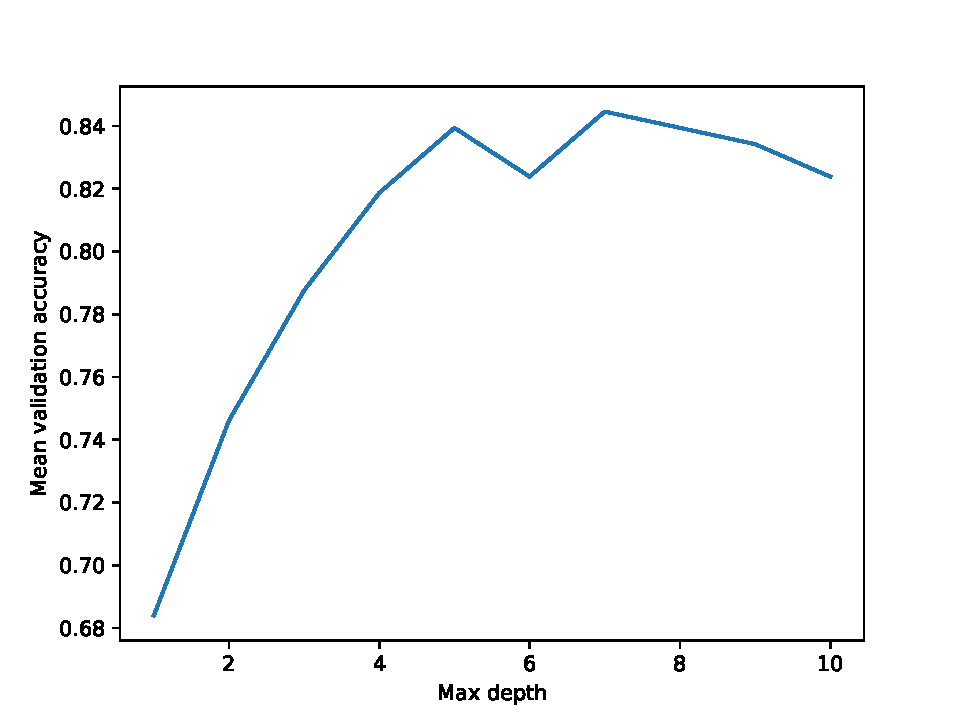
\includegraphics[width=0.9\textwidth]{../outputs/forest_classifier_validation.pdf}
    
\end{frame}
    

\subsection{Classifier testing ROC}
\begin{frame}{Classifier testing ROC}

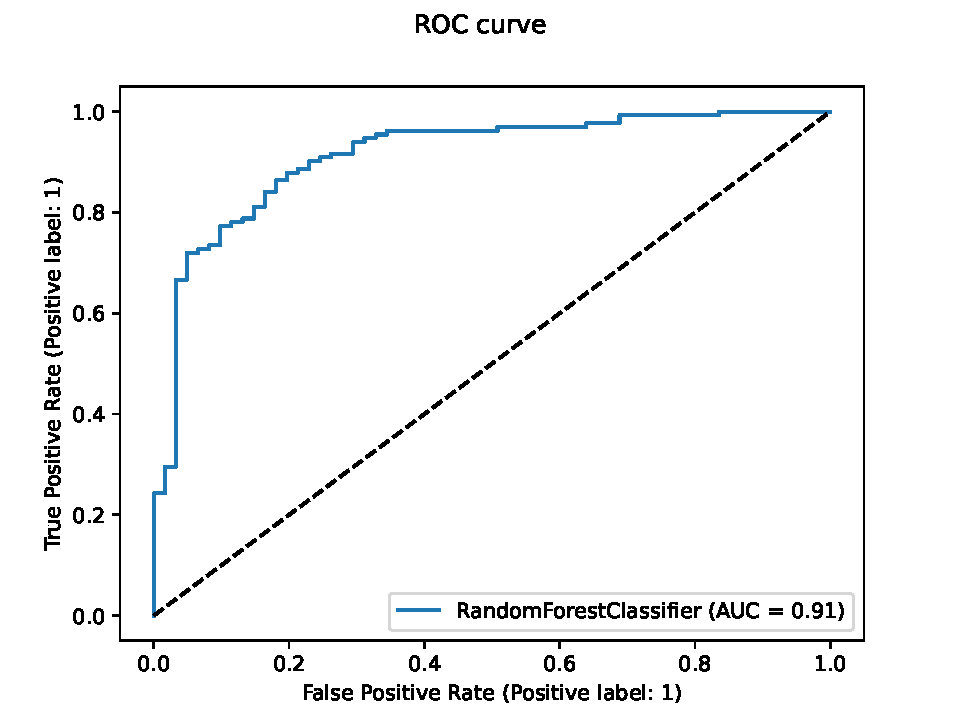
\includegraphics[width=0.9\textwidth]{../outputs/test_classification_plot.pdf}
    
\end{frame}
    

\subsection{Regressor paramter tuning}
\begin{frame}{Regressor paramter tuning}

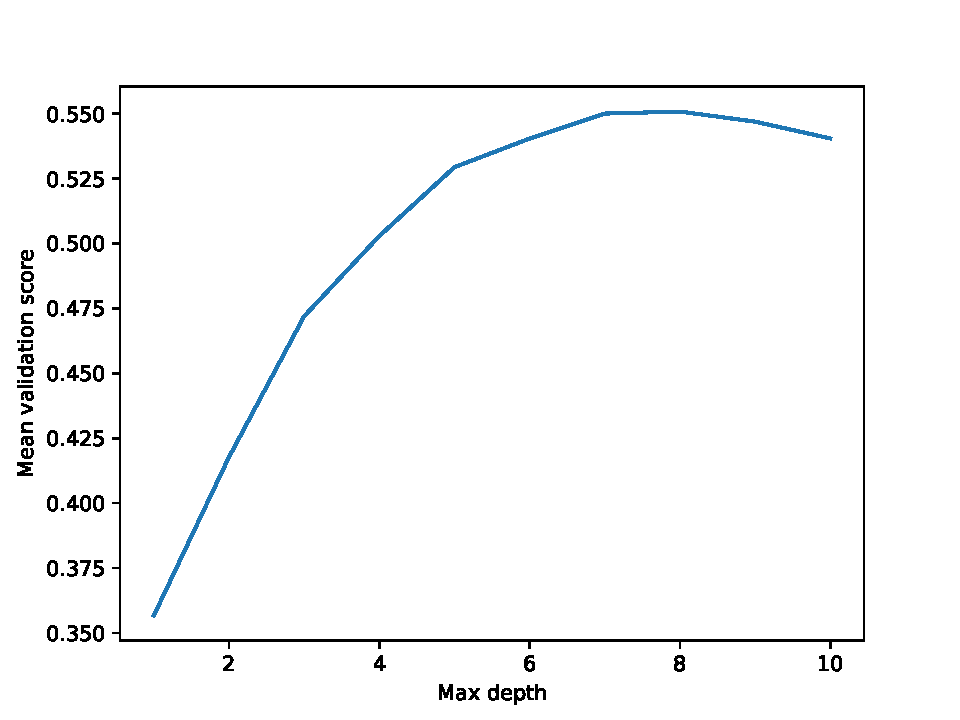
\includegraphics[width=0.9\textwidth]{../outputs/forest_regressor_validation.pdf}
    
\end{frame}
    

\subsection{Regressor testing residuals}
\begin{frame}{Regressor testing residuals}

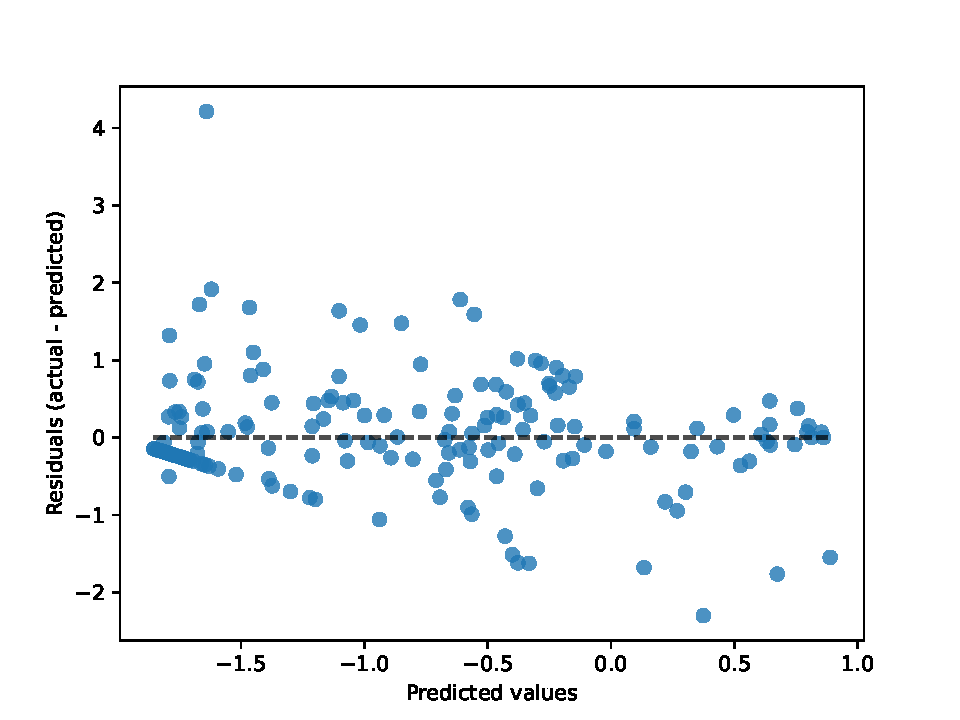
\includegraphics[width=0.9\textwidth]{../outputs/test_regression_plot.pdf}
    
\end{frame}
    

\end{document}
    